\documentclass[14pt, a4paper, twoside]{extreport}
\usepackage[utf8]{inputenc}
\usepackage{graphicx}
\usepackage[T2A]{fontenc}
\usepackage{geometry}
\usepackage{array}
\usepackage{graphicx}
\usepackage{setspace}
\usepackage{siunitx}
\usepackage{caption}
\usepackage{titlesec}
\usepackage[russian]{babel}
\usepackage{indentfirst}
\usepackage{setspace}
\usepackage{float}
\usepackage{array}
\usepackage{cellspace}
\usepackage{pgfplots}
\usepackage{pgfplotstable}
\usepackage{tocloft}
\usepackage{amsmath}
\usepackage{multirow}
\setlength{\cellspacetoplimit}{20pt}
\setlength{\cellspacebottomlimit}{20pt}

\onehalfspacing

\geometry{
  a4paper,
  left=30mm,
  right=20mm,
  top=20mm,
  bottom=20mm
}

\setlength{\parindent}{1.25cm}

\graphicspath{ {images/} }
\captionsetup[figure]{
  labelsep=period,
  justification=centering
}

\renewcommand{\figurename}{Рисунок}
\renewcommand{\contentsname}{\centering Оглавление}

\titleformat{\chapter}[block]{\huge\bfseries\centering}{}{1em}{}
\titleformat{\section}[block]{\normalsize\bfseries}{\thesection}{1em}{}
\titleformat{\subsection}[block]{\normalsize\bfseries}{\thesubsection}{1em}{}
\titlespacing*{\section}{0pt}{\parskip}{-\parskip}
\titlespacing*{\subsection}{0pt}{\parskip}{-\parskip}
\titlespacing{\chapter}{0pt}{-50pt}{0pt}

\renewcommand{\cftbeforetoctitleskip}{-30pt}
\renewcommand{\cftaftertoctitleskip}{-10pt}

\begin{document}

\begin{titlepage}
  \begin{center}
    \small
    \underline{
      \begin{minipage}{0.2\textwidth}
        \centering
        
\includegraphics[width=3cm]{BMSTU logo}
      \end{minipage}
      \hfill
      \begin{minipage}{0.8\textwidth}
        \begin{center}

          \textbf{Министерство науки и высшего образования Российской Федерации
            Федеральное государственное бюджетное образовательное учреждение высшего образования «Московский государственный технический университет имени Н.Э. Баумана национальный исследовательский университет»
          (МГТУ им. Н.Э. Баумана)}
        \end{center}
      \end{minipage}

    }

    \vspace{7cm}
    \Large
    \textbf{Лабораторная работа Э-2} \\
    "Электроизмерительные приборы в физической лаборатории"\\
    \vspace{5cm}
    \normalsize
    \begin{tabular}{p{8cm}p{6cm}}
      \textbf{Студент группы ИУ1-31Б} & \hrulefill \\
      & «\underline{\hspace{1.5cm}}»\underline{\hspace{2.5cm}}2025 г. \\
      & \\
      \textbf{Преподаватель} & \hrulefill \\
      & «\underline{\hspace{1.5cm}}»\underline{\hspace{2.5cm}}2025 г. \\
    \end{tabular}
    \vfill{\Large{Москва, 2025}}
  \end{center}
\end{titlepage}

\tableofcontents
\newpage

\chapter{Конспект}

\section{Введение}
Выполнение большинства лабораторных работ в физическом практикуме сопровождается измерением электрических величин, что позволяет изучить сущность исследуемого физического процесса или определить параметры установки.

\textbf{Основные средства измерений:}
\begin{itemize}
  \item Показывающие стрелочные и цифровые амперметры и вольтметры
  \item Универсальные цифровые вольтметры
  \item Универсальный осциллограф
  \item Генератор сигналов низкочастотный
\end{itemize}

\section{Классификация электроизмерительных приборов}
\begin{enumerate}
  \item \textbf{По функциональному признаку:}
    \begin{itemize}
      \item Собирающие, обрабатывающие и предоставляющие измерительную информацию
      \item Аттестующие и поверяющие
    \end{itemize}

  \item \textbf{По способу представления результатов:}
    \begin{itemize}
      \item Показывающие
      \item Регистрирующие
    \end{itemize}

  \item \textbf{По методу измерения:}
    \begin{itemize}
      \item Непосредственно оценивающие
      \item Сравнивающие
    \end{itemize}

  \item \textbf{По способу применения и конструкции:}
    \begin{itemize}
      \item Щитовые, переносные, стационарные
    \end{itemize}

  \item \textbf{По точности измерения:}
    \begin{itemize}
      \item Измерительные (нормируются погрешности)
      \item Индикаторные (внеклассные)
      \item Указывающие (погрешность не нормируется)
    \end{itemize}

  \item \textbf{По принципу действия:}
    \begin{itemize}
      \item Электромеханические, электронные, электрохимические
    \end{itemize}
\end{enumerate}

\section{Основные методы измерения электрических величин}

\subsection{Метод непосредственной оценки}
Проводят с помощью амперметров и вольтметров со стрелочным или цифровым отсчетом.

\begin{itemize}
  \item \textbf{Амперметры:} включают в разрыв цепи
    \begin{itemize}
      \item Собственное сопротивление $R_A$ должно быть мало
      \item Потребляемая мощность $P = R_A I^2_{\text{изм}}$ незначительна
    \end{itemize}

  \item \textbf{Вольтметры:} подключают параллельно
    \begin{itemize}
      \item Входное сопротивление $R_V$ должно быть большим
      \item Потребляемая мощность $P = \frac{U^2}{R_V}$ мала
    \end{itemize}
\end{itemize}

\subsection{Метод сравнения}
Позволяет измерять напряжение и ЭДС с высокой точностью. Используется в компенсационных схемах и электронных вольтметрах.

\textbf{Суть метода:} измеряемая величина сравнивается с напряжением высокостабильного источника, и в момент их равенства производится индикация.

\section{Основные характеристики электроизмерительных приборов}

\subsection{Основные параметры}
\begin{itemize}
  \item \textbf{Диапазон измерений} - область значений, для которой нормированы погрешности

  \item \textbf{Чувствительность:}
    \[
      E = \frac{dl}{dx} \quad \text{или} \quad E = \frac{d\phi}{dx}
    \]
    где $dl$, $d\phi$ - линейное и угловое перемещение указателя; $dx$ - изменение измеряемой величины.

  \item \textbf{Порог чувствительности} - минимальное изменение измеряемой величины, которое может быть зарегистрировано прибором

  \item \textbf{Цена деления шкалы:}
    \[
      C = \frac{dx}{dl} \quad \text{или} \quad C = \frac{dx}{d\phi}
    \]
    Обычно $C = 2\Delta$ или $C = 4\Delta$, где $\Delta$ - абсолютная погрешность.
\end{itemize}

\subsection{Погрешности и классы точности}

\subsubsection{Виды погрешностей}
\begin{itemize}
  \item \textbf{Абсолютная погрешность:}
    \[
      \Delta = x - a
    \]
    где $x$ - показание прибора, $a$ - действительное значение.

  \item \textbf{Относительная погрешность:}
    \[
      \varepsilon = \frac{\Delta}{a}
    \]

  \item \textbf{Приведенная погрешность:}
    \[
      \gamma = \frac{\Delta}{a_N}
    \]
    где $a_N$ - нормирующее значение.
\end{itemize}

\subsubsection{Класс точности}
\begin{itemize}
  \item \textbf{Определение:}
    \[
      K = \gamma_{\text{max}} \cdot 100\%
    \]

  \item \textbf{Классы по ГОСТ 1845-59:}
    \begin{itemize}
      \item 0,05; 0,1; 0,2 - образцовые приборы
      \item 0,5; 1,0 - лабораторные
      \item 1,5; 2,5; 4,0 - технические
    \end{itemize}

  \item \textbf{Максимальная абсолютная погрешность:}
    \[
      \Delta_{\text{max}} = \frac{a_N \cdot K}{100}
    \]

  \item \textbf{Оценка относительной погрешности:}
    \[
      \varepsilon \leq K \cdot \frac{a_N}{a \cdot 100} \approx K \cdot \frac{a_N}{x \cdot 100}
    \]
\end{itemize}

\subsection{Пример расчета погрешности}
Ток силой 2,5 А измеряют двумя амперметрами:
\begin{itemize}
  \item Класс точности 0,5, предел 25 А: $\varepsilon_1 = 0,5 \cdot \frac{25}{2,5 \cdot 100} = 0,05$
  \item Класс точности 1,0, предел 5 А: $\varepsilon_2 = 1,0 \cdot \frac{5}{2,5 \cdot 100} = 0,02$
\end{itemize}

Результаты измерений:
\[
  I_1 = (2,5 \pm 0,1)\ \text{А}; \quad I_2 = (2,50 \pm 0,05)\ \text{А}
\]

\section{Основные системы электромеханических приборов}

\subsection{Магнитоэлектрическая система}
\begin{figure}[H]
  \centering
  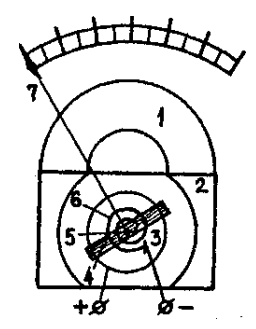
\includegraphics[width=0.6\textwidth]{magneto_electric.png}
  \caption{Измерительный механизм магнитоэлектрической системы}
  \label{fig:magneto_electric}
\end{figure}

\textbf{Принцип действия:} взаимодействие контура с током и магнитного поля постоянного магнита.

\textbf{Достоинства:}
\begin{itemize}
  \item Высокая чувствительность
  \item Большая точность (классы 0,05; 0,1; 0,2)
  \item Равномерная шкала
  \item Малое потребление энергии ($10^{-5}...10^{-6}$ Вт)
\end{itemize}

\textbf{Недостатки:}
\begin{itemize}
  \item Сложность устройства
  \item Невозможность измерения переменных токов
  \item Чувствительность к перегрузкам
\end{itemize}

\subsection{Электромагнитная система}
\begin{figure}[H]
  \centering
  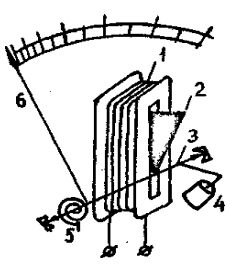
\includegraphics[width=0.6\textwidth]{electromagnetic.png}
  \caption{Измерительный механизм электромагнитной системы}
  \label{fig:electromagnetic}
\end{figure}

\textbf{Принцип действия:} взаимодействие магнитного поля катушки с магнитомягким сердечником.

\textbf{Особенности:}
\begin{itemize}
  \item Вращающий момент пропорционален квадрату тока: $M \sim I^2$
  \item Применяются для постоянного и переменного тока
  \item Шкала неравномерная (квадратичная)
  \item Классы точности: 1,0; 1,5; 2,5
\end{itemize}

\subsection{Электродинамическая система}
\textbf{Принцип действия:} взаимодействие двух контуров с токами.

\textbf{Особенности:}
\begin{itemize}
  \item Вращающий момент пропорционален произведению токов: $M \sim I_1 I_2$
  \item Применяются как амперметры, вольтметры и ваттметры
  \item Классы точности: 0,1; 0,2; 0,5
\end{itemize}

\subsection{Электростатическая система}
\textbf{Принцип действия:} взаимодействие электрически заряженных подвижных и неподвижных пластин.

\textbf{Достоинства:}
\begin{itemize}
  \item Очень большое входное сопротивление (10-100 МОм)
  \item Измеряют постоянные и переменные напряжения до $10^7...10^8$ Гц
  \item Не вносят искажений в исследуемую цепь
\end{itemize}

\section{Электронные цифровые вольтметры}

\subsection{Структурная схема}
\begin{figure}[H]
  \centering
  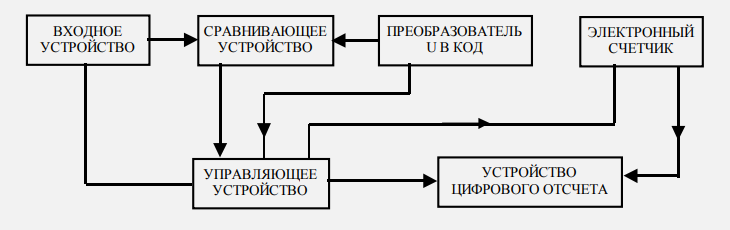
\includegraphics[width=0.8\textwidth]{digital_voltmeter.png}
  \caption{Обобщенная структурная схема электронного цифрового вольтметра}
  \label{fig:digital_voltmeter}
\end{figure}

\textbf{Основные узлы:}
\begin{itemize}
  \item Входное устройство (калиброванный делитель)
  \item Сравнивающее устройство
  \item Преобразователь напряжения в код
  \item Устройство цифрового отсчета
  \item Управляющее устройство
\end{itemize}

\subsection{Принцип действия времяимпульсного преобразователя}
\begin{figure}[H]
  \centering
  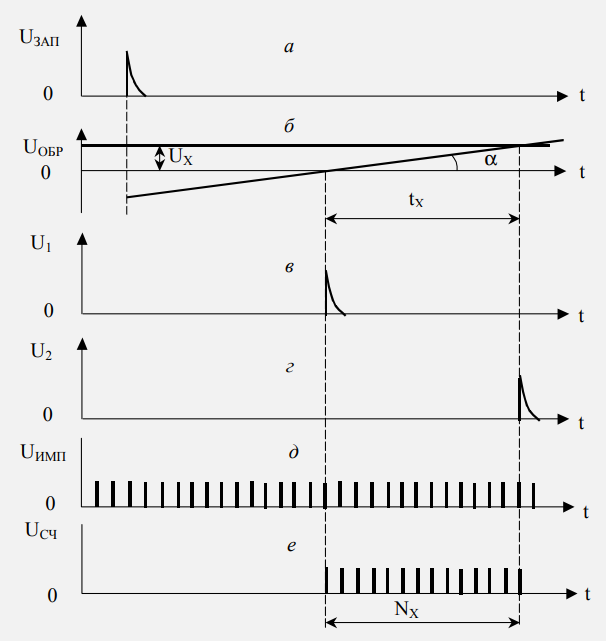
\includegraphics[width=0.9\textwidth]{time_diagram.png}
  \caption{Временная диаграмма работы времяимпульсного вольтметра}
  \label{fig:time_diagram}
\end{figure}

Измеряемое напряжение преобразуется во временной интервал:
\[
  U_X = t_X \cdot \nu = \eta \cdot N_X
\]
где $\eta = \frac{\nu}{V_0}$ - постоянный коэффициент, $N_X$ - число импульсов.

\section{Универсальный осциллограф}

\subsection{Структурная схема}
\begin{figure}[H]
  \centering
  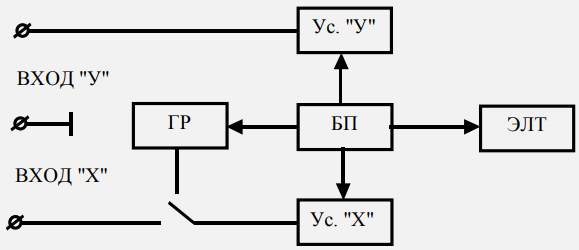
\includegraphics[width=0.8\textwidth]{oscilloscope.png}
  \caption{Структурная схема универсального осциллографа}
  \label{fig:oscilloscope}
\end{figure}

\textbf{Основные блоки:}
\begin{itemize}
  \item Электронно-лучевая трубка (ЭЛТ)
  \item Генератор развертки
  \item Усилитель вертикального отклонения (Y)
  \item Усилитель горизонтального отклонения (X)
  \item Блок питания
\end{itemize}

\subsection{Электронно-лучевая трубка}
\begin{figure}[H]
  \centering
  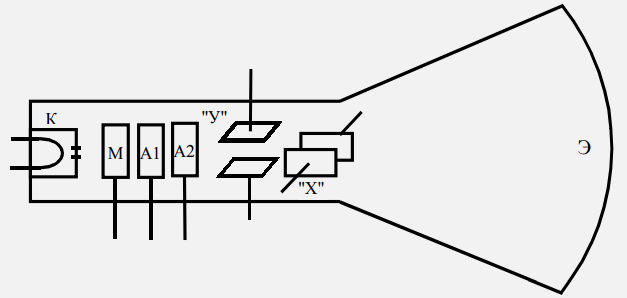
\includegraphics[width=0.7\textwidth]{crt.png}
  \caption{Устройство электронно-лучевой трубки}
  \label{fig:crt}
\end{figure}

\textbf{Основные элементы:}
\begin{itemize}
  \item Катод (К) - источник электронов
  \item Модулятор (М) - управление плотностью луча
  \item Аноды (A1, A2) - ускорение и фокусировка
  \item Отклоняющие пластины (X, Y)
  \item Экран с люминофором
\end{itemize}

\subsection{Чувствительность пластин}
Чувствительность пластин к напряжению:
\[
  \ae = \frac{h}{U}
\]
где $h$ - смещение пятна на экране, $U$ - приложенное напряжение.

Коэффициент отклонения:
\[
  b = \frac{1}{\ae}
\]

\subsection{Фигуры Лиссажу}
\begin{figure}[H]
  \centering
  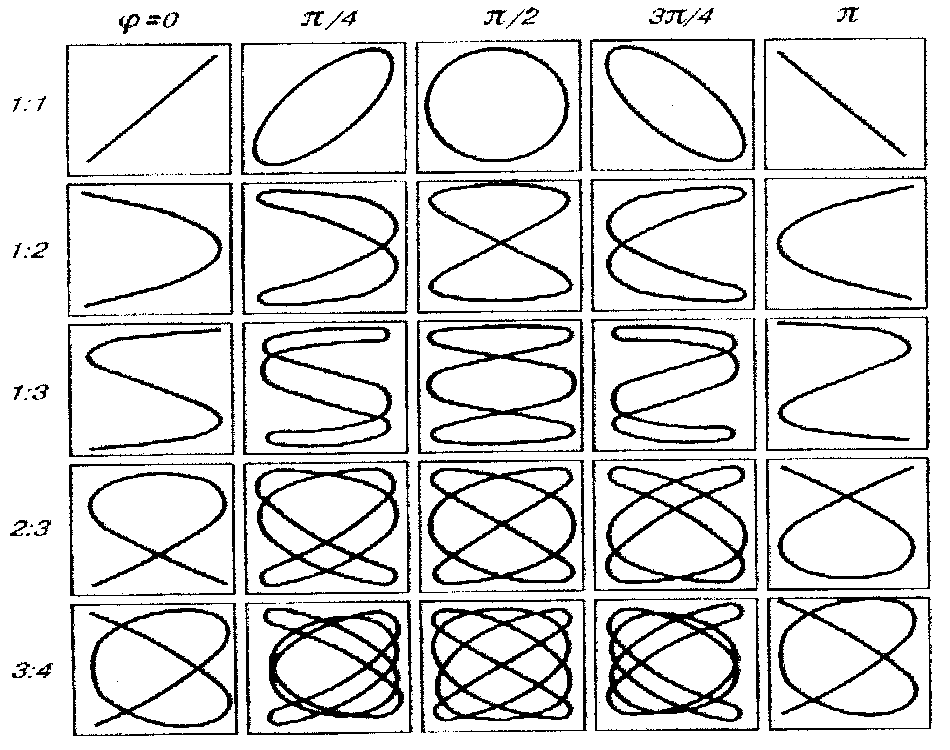
\includegraphics[width=0.8\textwidth]{lissajous.png}
  \caption{Фигуры Лиссажу для различных соотношений частот и фаз}
  \label{fig:lissajous}
\end{figure}

\textbf{Определение частоты:}
\[
  \frac{\nu_y}{\nu_x} = \frac{n_x}{n_y}
\]
где $n_x$, $n_y$ - числа пересечений фигуры с горизонтальной и вертикальной прямыми.

\section{Универсальный цифровой вольтметр В7-27}

\subsection{Назначение и технические данные}
\begin{itemize}
  \item \textbf{Назначение:} измерение постоянного и переменного напряжений, постоянного тока, сопротивления и температуры
  \item \textbf{Погрешность измерения переменного напряжения:}
    \[
      \varepsilon = \left[1 + 0,5\left(\frac{U_k}{U} - 1\right)\right]\%
    \]
    где $U_k$ - значение установленного предела измерения, $U$ - измеряемое значение
  \item \textbf{Диапазон:} от 100 мВ до 1000 В, частоты 20 Гц - 100 кГц
\end{itemize}

\subsection{Порядок подготовки к измерениям}
\begin{enumerate}
  \item Ознакомиться с переключателями управления
  \item Включить тумблер "Сеть"
  \item Установить нулевое показание:
    \begin{itemize}
      \item Установить предел измерения
      \item Замкнуть входные гнезда
      \item Установить "0" переменным резистором
    \end{itemize}
  \item Подать сигнал от объекта измерения
  \item Считать результат с индикаторного табло
  \item При перегрузке (символ "П" или ">") отсоединить вольтметр
\end{enumerate}

\section{Генератор сигналов низкочастотный ГЗ-102}

\subsection{Назначение и технические данные}
\begin{itemize}
  \item \textbf{Назначение:} источник синусоидальных колебаний звукового и ультразвукового диапазонов
  \item \textbf{Диапазон частот:} 20 Гц - 200 кГц (4 поддиапазона)
  \item \textbf{Погрешность по частоте:}
    \[
      \varepsilon_\nu = \left(1 + \frac{50}{\sqrt{\nu}}\right)\% \quad \text{(20 Гц - 20 кГц)}
    \]
    \[
      \varepsilon_\nu = 1,5\% \quad \text{(20 - 200 кГц)}
    \]
  \item \textbf{Выходная мощность:} не менее 100 мВт (7,75 В)
  \item \textbf{Максимальное выходное напряжение:} 8 В
\end{itemize}

\subsection{Структурная схема}
\begin{figure}[H]
  \centering
  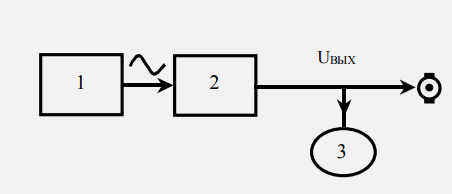
\includegraphics[width=0.6\textwidth]{generator_scheme.png}
  \caption{Структурная схема генератора ГЗ-102}
  \label{fig:generator_scheme}
\end{figure}

\textbf{Основные узлы:}
\begin{itemize}
  \item Задающий генератор 1
  \item Выходной усилитель 2 (буферное устройство)
  \item Индикатор напряжения 3
\end{itemize}

\section{Маркировка электроизмерительных приборов}

\subsection{Основные обозначения}
\begin{itemize}
  \item \textbf{Измеряемая величина:} mA (мА), µV (мкВ) и т.д.
  \item \textbf{Класс точности:} число на шкале (например, 0,5)
  \item \textbf{Род и частота тока:}
    \begin{itemize}
      \item Постоянный ток: ---
      \item Переменный ток: $\sim$
      \item Постоянный и переменный: $\approx$
      \item Диапазон частот: 45-550 Hz
    \end{itemize}
\end{itemize}

\subsection{Системы приборов и защищенность}
\begin{table}[H]
  \centering
  \begin{tabular}{|c|l|}
    \hline
    \textbf{Обозначение} & \textbf{Система} \\
    \hline
    \begin{minipage}{0.3\textwidth}
      \centering
      
\includegraphics[width=0.2\textwidth]{magneto_icon.png}
    \end{minipage} & Магнитоэлектрическая \\
    \hline
    \begin{minipage}{0.3\textwidth}
      \centering
      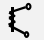
\includegraphics[width=0.2\textwidth]{electromagnetic_icon.png}
    \end{minipage} & Электромагнитная \\
    \hline
  \end{tabular}
  \caption{Обозначения систем приборов}
\end{table}

\subsection{Категории защищенности}
\begin{itemize}
  \item \textbf{I категория:} меньшая дополнительная погрешность от внешних полей
  \item \textbf{II категория:} обычная защищенность
\end{itemize}

\subsection{Рабочее положение}
\begin{itemize}
  \item Горизонтальное: $\rightarrow$
  \item Вертикальное: $\uparrow$
  \item Наклонное (40°): $\nearrow$
\end{itemize}

\subsection{Температурные группы}
\begin{table}[H]
  \centering
  \begin{tabular}{|c|c|c|}
    \hline
    \textbf{Группа} & \textbf{Температура, °C} & \textbf{Влажность, \%} \\
    \hline
    А & +10...+35 & до 80 \\
    Б & -30...+40 & до 90 \\
    В1 & -40...+50 & до 95 \\
    В2 & -50...+60 & до 95 \\
    В3 & -50...+80 & до 98 \\
    \hline
  \end{tabular}
  \caption{Температурные группы приборов}
\end{table}

\subsection{Устойчивость к механическим воздействиям}
\begin{itemize}
  \item Обыкновенный (без обозначения)
  \item ОП - обыкновенный с повышенной прочностью
  \item ТП - тряскопрочный
  \item ВП - вибропрочный
  \item ТН - нечувствительный к тряске
  \item ВН - нечувствительный к вибрациям
  \item УП - ударопрочный
  \item Бз - брызгозащищенный
  \item Вз - водозащищенный
  \item Гм - герметический
\end{itemize}

\section{Дополнения к теории измерений}

\subsection{Принцип компенсационного измерения}
\begin{itemize}
  \item Измеряемая величина сравнивается с образцовой
  \item В момент равенства производится фиксация результата
  \item Позволяет достигать высокой точности (0.01-0.005\%)
\end{itemize}

\subsection{Преимущества цифровых приборов}
\begin{itemize}
  \item Широкий диапазон измерений (мкВ - кВ)
  \item Высокое быстродействие
  \item Малые погрешности
  \item Отсутствие погрешности считывания
  \item Автоматизация измерений
\end{itemize}

\subsection{Требования к включению приборов}
\begin{table}[H]
  \centering
  \begin{tabular}{|l|l|l|}
    \hline
    \textbf{Прибор} & \textbf{Включение} & \textbf{Требования} \\
    \hline
    Амперметр & Последовательно & $R_A \ll R_{\text{цепи}}$ \\
    Вольтметр & Параллельно & $R_V \gg R_{\text{участка}}$ \\
    \hline
  \end{tabular}
  \caption{Правила включения измерительных приборов}
\end{table}

\subsection{Расчетные соотношения для цепей переменного тока}
\begin{itemize}
  \item \textbf{Действующее значение:} $I = \frac{I_m}{\sqrt{2}}$, $U = \frac{U_m}{\sqrt{2}}$
  \item \textbf{Мощность в цепи:} $P = UI\cos\varphi$
  \item \textbf{Резонансная частота:} $f_0 = \frac{1}{2\pi\sqrt{LC}}$
\end{itemize}

\chapter{Выполнение работы}
\section{Изучение RC-цепочки}

По результатам измерений были получены данные представленные в следующей таблице и на графике.

\begin{table}[H]
  \centering
  \begin{tabular}{|l|ll|}
    \hline
    \multirow{2}{*}{\textbf{Частота $\nu$, Гц}} & \multicolumn{2}{l|}{\textbf{Напряжение, В}}           \\ \cline{2-3}
    & \multicolumn{1}{l|}{\textbf{$U_R$}} & \textbf{$U_C$} \\ \hline
    100                               & \multicolumn{1}{l|}{1,003}         & 6,51          \\ \hline
    200                               & \multicolumn{1}{l|}{1,962}         & 6,28          \\ \hline
    300                               & \multicolumn{1}{l|}{2,747}         & 5,99          \\ \hline
    400                               & \multicolumn{1}{l|}{3,405}         & 5,64          \\ \hline
    500                               & \multicolumn{1}{l|}{4,00}          & 5,29          \\ \hline
    600                               & \multicolumn{1}{l|}{4,45}          & 4,97          \\ \hline
    700                               & \multicolumn{1}{l|}{4,80}          & 4,66          \\ \hline
    800                               & \multicolumn{1}{l|}{5,12}          & 4,35          \\ \hline
    900                               & \multicolumn{1}{l|}{5,35}          & 4,12          \\ \hline
    1000                              & \multicolumn{1}{l|}{5,53}          & 3,817         \\ \hline
    1100                              & \multicolumn{1}{l|}{5,71}          & 3,626         \\ \hline
    1200                              & \multicolumn{1}{l|}{5,87}          & 3,454         \\ \hline
    1300                              & \multicolumn{1}{l|}{6,00}          & 3,283         \\ \hline
    1400                              & \multicolumn{1}{l|}{6,11}          & 3,148         \\ \hline
    1500                              & \multicolumn{1}{l|}{6,2}           & 3,03          \\ \hline
  \end{tabular}
\end{table}

\begin{figure}[H]
  \centering
  \begin{tikzpicture}
    \begin{axis}[
        width=0.8\textwidth,
        height=0.4\textwidth,
        xlabel={Частота $\nu$, Гц},
        ylabel={Напряжение $U$, В},
        xmin=0, xmax=1600,
        ymin=0, ymax=7,
        grid=both,
        grid style={line width=.1pt, draw=gray!10},
        major grid style={line width=.2pt,draw=gray!50},
        legend pos= south east,
        legend cell align={left},
        title={Зависимости $U_R(\nu)$ и $U_C(\nu)$ для RC-цепи},
        xlabel style={font=\normalsize},
        ylabel style={font=\normalsize}
      ]

      % Данные для U_R
      \addplot[
        color=blue,
        mark=*,
        mark size=1.5pt,
        line width=1.2pt
      ] coordinates {
        (100, 1.003)
        (200, 1.962)
        (300, 2.747)
        (400, 3.405)
        (500, 4.00)
        (600, 4.45)
        (700, 4.80)
        (800, 5.12)
        (900, 5.35)
        (1000, 5.53)
        (1100, 5.71)
        (1200, 5.87)
        (1300, 6.00)
        (1400, 6.11)
        (1500, 6.2)
      };
      \addlegendentry{$U_R$ (напряжение на резисторе)}

      % Данные для U_C
      \addplot[
        color=red,
        mark=square*,
        mark size=1.5pt,
        line width=1.2pt
      ] coordinates {
        (100, 6.51)
        (200, 6.28)
        (300, 5.99)
        (400, 5.64)
        (500, 5.29)
        (600, 4.97)
        (700, 4.66)
        (800, 4.35)
        (900, 4.12)
        (1000, 3.817)
        (1100, 3.626)
        (1200, 3.454)
        (1300, 3.283)
        (1400, 3.148)
        (1500, 3.03)
      };
      \addlegendentry{$U_C$ (напряжение на конденсаторе)}

      % Добавим пунктирные линии для резонансной частоты (примерно 1000 Гц)
      \draw[dashed, gray] (1000,0) -- (1000,7);
      \node[anchor=north] at (1000,0.2) {$\nu_0 \approx 1000$ Гц};

    \end{axis}
  \end{tikzpicture}
  \caption{Зависимости напряжений на резисторе $U_R$ и конденсаторе $U_C$ от частоты в RC-цепи}
  \label{fig:ur_uc}
\end{figure}

\section{Работа с осцилографом}
Результаты измерений
\begin{table}[H]
  \centering
  \begin{tabular}{|l|l|l|l|l|l|}
    \hline
    \textbf{Величина}            & l          & n     & $\tau_p$       & y            & b \\ \hline
    \textbf{Результат измерений} & 0.0721 м   & 3     & 0.002 с        & 0.056 м      & 5 В/м         \\ \hline
  \end{tabular}
\end{table}

Вычисление периода и частоты синусоиды
\begin{equation}
  T = \frac{l\tau_p}{n} = \frac{0.0721 \cdot 0.002}{3} = 4.807 \text{мс}
\end{equation}

\begin{equation}
  \nu = \frac{1}{T} = \frac{1}{4.807\cdot 10^{(-3)} } = 208.044 \text{Гц}
\end{equation}

\section{Фигуры Лиссажу}
\subsection{Результаты экспериментов}

\begin{table}[H]
  \centering
  \begin{tabular}{|c|c|c|c|}
    \hline
    № опыта & $\nu_x$:$\nu_y$ & Вид фигуры & Параметры \\
    \hline
    1 & 1:1 & 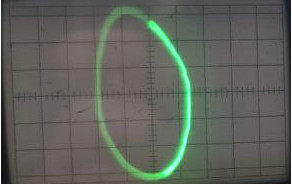
\includegraphics[width=0.15\textwidth]{lissajous1-1.jpg} & Эллипс/окружность \\
    \hline
    2 & 2:1 & 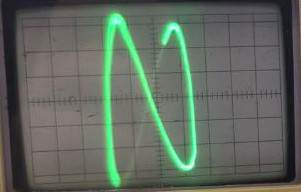
\includegraphics[width=0.15\textwidth]{lissajous1-2.jpg} & "Восьмерка" \\
    \hline
    3 & 3:1 & 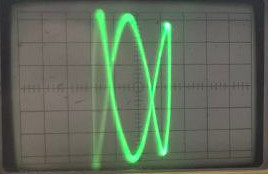
\includegraphics[width=0.15\textwidth]{lissajous1-3.jpg} & Сложная фигура \\
    \hline
  \end{tabular}
  \caption{Наблюдаемые фигуры Лиссажу}
\end{table}

\subsection{Анализ результатов}

\subsubsection{Опыт 1 ($\nu_x : \nu_y = 1:1$)}
\begin{itemize}
  \item \textbf{Наблюдается:} эллипс, окружность или наклонная прямая
  \item \textbf{Форма зависит от разности фаз $\Delta\phi = \phi_2 - \phi_1$:}
    \begin{itemize}
      \item $\Delta\phi = 0$: прямая $y = \frac{B}{A}x$ (I и III квадранты)
      \item $\Delta\phi = \pi$: прямая $y = -\frac{B}{A}x$ (II и IV квадранты)
      \item $\Delta\phi = \frac{\pi}{2}$: эллипс $\frac{x^2}{A^2} + \frac{y^2}{B^2} = 1$
      \item $A = B$, $\Delta\phi = \frac{\pi}{2}$: окружность $x^2 + y^2 = A^2$
    \end{itemize}
\end{itemize}

\subsubsection{Опыт 2 ($\nu_x : \nu_y = 2:1$)}
\begin{itemize}
  \item \textbf{Наблюдается:} фигура в виде "восьмерки" или "скобки"
  \item \textbf{Объяснение:} за время одного периода колебаний по Y, по X совершается два полных периода
  \item Фигура более сложной формы, замкнутая
\end{itemize}

\subsubsection{Опыт 3 ($\nu_x : \nu_y = 3:1$)}
\begin{itemize}
  \item \textbf{Наблюдается:} сложная фигура с тремя петлями
  \item \textbf{Объяснение:} за время одного периода по Y, по X совершается три полных периода
  \item Форма зависит от начальных фаз колебаний
\end{itemize}

\subsection{Определение параметров сигналов}

\subsubsection{Определение соотношения частот}
\begin{itemize}
  \item Провести горизонтальную и вертикальную прямые, пересекающие фигуру
  \item Посчитать число пересечений:
    \begin{itemize}
      \item $n_x$ -- с горизонтальной прямой
      \item $n_y$ -- с вертикальной прямой
    \end{itemize}
  \item \textbf{Формула для соотношения частот:}
    \[
      \frac{\nu_y}{\nu_x} = \frac{n_x}{n_y}
    \]
\end{itemize}

\subsubsection{Определение разности фаз}
\begin{itemize}
  \item Для случая $\nu_x = \nu_y$ по форме эллипса можно определить $\Delta\phi$:
    \[
      \sin(\Delta\phi) = \frac{y_0}{B} = \frac{x_0}{A}
    \]
    где $y_0$, $x_0$ -- координаты пересечения эллипсом осей
\end{itemize}

\subsubsection{Определение амплитуд}
\begin{itemize}
  \item По максимальным отклонениям по осям X и Y определяются амплитуды сигналов:
    \[
      A = x_{\text{max}}, \quad B = y_{\text{max}}
    \]
\end{itemize}

\subsection{Выводы}

\begin{enumerate}
  \item Фигуры Лиссажу позволяют определять соотношение частот двух гармонических сигналов
  \item При равенстве частот можно определить разность фаз между сигналами
  \item Форма фигуры зависит от соотношения частот, амплитуд и разности фаз
  \item Метод особенно полезен для сравнения частот высокочастотных сигналов
  \item Точность определения частоты повышается с увеличением числа пересечений фигуры с осями
\end{enumerate}

\chapter{Контрольные вопросы}

\section{По каким признакам классифицируются электроизмерительные приборы?}

\begin{itemize}
  \item По функциональному признаку (собирающие, обрабатывающие, предоставляющие измерительную информацию)
  \item По способу представления результатов (показывающие и регистрирующие)
  \item По методу измерения (непосредственно оценивающие и сравнивающие)
  \item По способу применения и конструкции (щитовые, переносные, стационарные)
  \item По точности измерения (измерительные, индикаторные, указывающие)
  \item По принципу действия (электромеханические, электронные, электрохимические)
\end{itemize}

\section{Перечислите основные методы измерения электрических величин.}

\begin{itemize}
  \item \textbf{Метод непосредственной оценки} -- с помощью амперметров и вольтметров
  \item \textbf{Метод сравнения} -- сравнение измеряемой величины с образцовой
\end{itemize}

\section{Что такое класс точности прибора?}

Класс точности $K$ -- обобщенная характеристика, определяющая пределы допустимых погрешностей:
\[
  K = \gamma_{\text{max}} \cdot 100\%
\]
где $\gamma_{\text{max}}$ -- максимальная приведенная погрешность.

\section{Как определить относительную погрешность измерения по показанию стрелочного прибора?}

Относительная погрешность определяется по формуле:
\[
  \varepsilon \leq K \cdot \frac{a_N}{x \cdot 100}
\]
где $K$ -- класс точности, $a_N$ -- нормирующее значение, $x$ -- показание прибора.

\section{Как получить более высокую точность измерения тока или напряжения, пользуясь многопредельным прибором?}

\begin{itemize}
  \item Выбирать предел измерения, близкий к значению измеряемой величины
  \item Использовать прибор с более высоким классом точности
  \item Работать в средней части шкалы прибора
\end{itemize}

\section{В чем состоит принцип работы приборов электромагнитной и магнитоэлектрической систем?}

\begin{itemize}
  \item \textbf{Магнитоэлектрическая:} взаимодействие контура с током и магнитного поля постоянного магнита
  \item \textbf{Электромагнитная:} взаимодействие магнитного поля катушки с ферромагнитным сердечником
\end{itemize}

\section{Какую информацию можно получить на основе условных обозначений, приводимых на шкале?}

\begin{itemize}
  \item Измеряемую величину и единицы измерения
  \item Класс точности
  \item Род тока (--, $\sim$, $\approx$)
  \item Систему прибора
  \item Рабочее положение
  \item Испытательное напряжение
  \item Температурную группу
\end{itemize}

\section{Что такое цена деления шкалы?}

Цена деления -- изменение измеряемой величины, вызывающее перемещение указателя на одно деление:
\[
  C = \frac{dx}{dl} \quad \text{или} \quad C = \frac{dx}{d\phi}
\]

\section{Изложите принцип работы цифрового вольтметра с времяимпульсным преобразованием.}

\begin{itemize}
  \item Измеряемое напряжение преобразуется во временной интервал
  \item Интервал заполняется счетными импульсами
  \item Импульсы подсчитываются электронным счетчиком
  \item Результат отображается в цифровой форме
\end{itemize}

\section{Какова структурная схема генератора ГЗ-102?}

\begin{itemize}
  \item Задающий генератор
  \item Выходной усилитель
  \item Индикатор напряжения
\end{itemize}

\section{Как измерить постоянное напряжение и ток при помощи вольтметра В7-27?}

\begin{enumerate}
  \item Установить соответствующий предел измерения
  \item Для напряжения: подключить к гнездам $U$ и $O$
  \item Для тока: подключить к гнездам $I$ и $O$
  \item Установить нулевое показание
  \item Считать результат с индикаторного табло
\end{enumerate}

\section{Каким образом оценивается погрешность измерения тока и напряжения вольтметром В7-27?}

Для переменного напряжения:
\[
  \varepsilon = \left[1 + 0,5\left(\frac{U_k}{U} - 1\right)\right]\%
\]
где $U_k$ -- предел измерения, $U$ -- измеряемое значение.

\section{Каково назначение осциллографа?}

\begin{itemize}
  \item Визуальное наблюдение электрических сигналов
  \item Измерение параметров сигналов (амплитуда, период, частота)
  \item Исследование формы сигналов
\end{itemize}

\section{Назовите основные узлы осциллографа.}

\begin{itemize}
  \item Электронно-лучевая трубка (ЭЛТ)
  \item Генератор развертки
  \item Усилитель вертикального отклонения (Y)
  \item Усилитель горизонтального отклонения (X)
  \item Блок питания
\end{itemize}

\section{Расскажите об устройстве электронно-лучевой трубки.}

\begin{itemize}
  \item Катод с подогревателем -- источник электронов
  \item Модулятор -- управление плотностью луча
  \item Аноды -- ускорение и фокусировка электронов
  \item Отклоняющие пластины X и Y
  \item Экран с люминофором
\end{itemize}

\section{От чего зависит чувствительность пластин?}

\begin{itemize}
  \item Геометрии пластин
  \item Расположения пластин относительно друг друга и экрана
  \item Скорости электронов
  \item Напряжения на ускоряющих электродах
\end{itemize}

\section{Почему чувствительность пластин X и Y неодинакова?}

\begin{itemize}
  \item Разное расстояние до экрана
  \item Разная геометрия пластин
  \item Разное расположение в пространстве трубки
  \item Разная емкость и индуктивность
\end{itemize}

\section{Каково назначение генератора пилообразного напряжения?}

\begin{itemize}
  \item Создание линейно нарастающего напряжения
  \item Обеспечение горизонтальной развертки луча
  \item Синхронизация с исследуемым сигналом
\end{itemize}

\section{Как определить частоту исследуемого напряжения методом фигур Лиссажу?}

\begin{itemize}
  \item Подать сигналы на пластины X и Y
  \item Зарисовать фигуру Лиссажу
  \item Провести горизонтальную и вертикальную прямые
  \item Посчитать число пересечений:
    \[
      \frac{\nu_y}{\nu_x} = \frac{n_x}{n_y}
    \]
    где $n_x$, $n_y$ -- числа пересечений с горизонтальной и вертикальной прямыми
\end{itemize}

\end{document}
\end{document}